\documentclass[draftclsnofoot,onecolumn,journal,letterpaper,compsoc,10pt]{IEEEtran}
\usepackage{geometry}
\usepackage{setspace}
\usepackage{color}
\usepackage{titling}
\usepackage{pdfpages}
\usepackage{float}

% ------ Removes the automatic references header ------
\usepackage{etoolbox}
\patchcmd{\thebibliography}{\section*{\refname}}{}{}{}
% -----------------------------------------------------

\geometry{letterpaper, margin=.75in}
\singlespace

\date{October 23, 2018}

\begin{document}

% Title Page + Abstract
\begin{titlingpage}
    \title{Software Requirments\\\large CS 461 Fall 2018}
    \author{
        Brennan Douglas \\
        \texttt{douglbre@oregonstate.edu} \\
        \and
        Dan Van Horn \\
        \texttt{vanhornd@oregonstate.edu} \\
        \and
        Henry Peterson \\
        \texttt{peterhen@oregonstate.edu} \\
        \and
        Bailey Singleton \\
        \texttt{singletb@oregonstate.edu} \\
    }
    \maketitle
    \begin{abstract}
    	During the brewing of a batch of beer there are many variables that need to be tested and tracked. This helps determine when the beer is ready and how it compares to other batches. Ninkasi --- a brewery in Eugene, Oregon --- is using a single large excel spreadsheet to track and store all their information. As they have grown, this has become increasingly unwieldy. There is already the beginning of a solution which includes a small set of applications designed to manage this data automatically while allowing for editing and visualization. This system will manage brewing data and user permissions to reduce the possibility for human error. The system needs to be hosted on a cloud provider and designed to be both desktop and mobile compatible.
    \end{abstract}
    \pagebreak
    \tableofcontents
\end{titlingpage}

\section{Introduction}

This document will lay out the technical specifications for the completion of the Ninkasi project.  It will outline uses cases for new features, and features that need to be repaired or updated.  In total, this document will detail all that needs to be done in order for the automated brewing project to be considered complete.

    \subsection{System Purpose}

    The purpose of the automated brewing project is to make a more sustainable system for Ninkasi to track, store, and visualize the data associated with the brewing of their beer.  As it stands there is already an application that has a working database that models the data needed by Ninkasi and has some rudimentary pages to display and enter this data.  Our extension on the system has the purpose to improve on the existing application in all manner.
    
    Upon completion the application should allow users to enter data for a given beer batch on a mobile device.  This data will then be automatically added to a set of graphs to help visualize the stage at which the specific batch is through its life cycle.  The application will track all data history associated with these batches, the tanks, they are in, and the brand they are a part of.  This will allow deep analytic looks into the brewing process over years worth of data.
    
    \subsection{System Scope}
    
    The system stores all the data, both current and past, associated with each batch of beer that Ninkasi brews.  This is stored in a database.  The web application serves two purposes: to manage the data, and to display the data.  As data management is concerned this means adding and updating data.  Along with this will be a concept of user roles, so a basic login and security system is set in place.  An extension that this project adds is the importing of data from their alkalizer machine, in the form of CSV files.  This project also adds new forms of data visualization.  Specifically new graphs that represent the data in new light.  The final thing that this iteration on the application brings is an upgrade of the technologies being used to bring them to modern standards.  These are broken down into three epics:
    
    \begin{itemize}
        \item Maintenance 
        \item Data Flow
        \item User Interface
    \end{itemize}
    
    \subsection{System Overview}
    
        \subsubsection{System context}
        Previously Ninkasi was using large ever expanding excel spreadsheets to keep track of all of their data.  This single spreadsheet would be passed around by email to different people who would add data and make edits to newly entered data.  As their operation grew larger this has become more and more cumbersome and prone to errors.
    
        \subsubsection{System functions}
        The system stands to improve this process via the web application.  As the current application stands it isn't production ready.  Thus the Maintenance epic will fix this by improving and fixing different features while creating a more complete docker-ized version of the application.  From there the Data Flow through, mainly into, the application will be improved by adding some new features to allow quicker data entry.  Finally, the User Interface will be improved to allow for easier use and better understanding of the website.
        
        \subsubsection{User characteristics}
        There are two sets of users: the admin and the standard user.  The admin will be able to manage all other users and every faucet of the applications data.  They will be on par with a manger who is overseeing the brewing process for a particular brand, or more than one.  The standard user will then be the tester two makes the measurements on each batch and inputs the data.  They will be able to enter data and see the visualizations but won't have much control over the application.
        
        The user of this application, Ninkasi, is looking for it to be a streamlined data entry and visualization process.  It needs to be easy to use when a desktop computer isn't available as most of the data will be entered via a tablet carried around in one of their warehouses.  Past that they are looking for some parts of the process to be automated as well given how repetitive they are.

    \subsection{Definitions}
    \begin{itemize}
        \item We --- refers to our team name BrewHops
        \item Epic --- a big chunk of work that has one common objective.
        \item User Story --- a simple description of a software feature from an end-user perspective.
        \item Agile Software Development --- an approach to software development under which requirements and solutions evolve through the collaborative effort of self-organizing and cross-functional teams and their customer(s)/end user(s)
        \item Docker --- a container platform for normalizing the application's run-time environment \cite{docker}
        \item Kubernetes --- a container (e.g. docker) scripting platform \cite{kubernetes}
        \item K8 --- shorthand for Kubernetes
        \item React --- the web framework that the project uses \cite{react}
        \item TypeScript --- a typed version of JavaScript \cite{typescript}
    \end{itemize}

\section{References}
\bibliographystyle{IEEEtran}
\bibliography{./ref}

\section{System Requirements}
    \subsection{Functional Requirements}
    The function of the system is to track all of the brewing data that is currently tracked via excel spreadsheets. This data will be managed by form entry on a website and by an automated upload process.
    \subsection{Usability Requirements}
    The system must have a user friendly interface that is easy to navigate and needs little direction on how to use. There should be little chance for a user to make a mistake and all user input should have helpful validation messages.
    \subsection{System Security}
    Only authenticated users will be able to log into the system and view or make changes. This will be managed by JSON web tokens which will validate each request and all user input will be sanitized before sending it back to the server.
    \subsection{Information Management}
    The data will be stored in a PostGreSQL database running inside of a virtual machine. We will have redeploy scripts and and an archival process by which no data will be lost.
\section{Software Development Requirements}
        The software development requirements are organized into epics and further into user stories. As we will be adhering to agile software development methods, the layout of this section most accurately represents what work will be completed and how it will be organized. Each "story" is written in the context of the party to whom the task benefits.
    \subsection{Maintenance}
        \subsubsection{Login process}
        The login process for the application is not working currently and there are currently only administrator roles available. As a user, there must be a secure way to log into the system and there must be appropriate administrator and non-administrator privileges assigned to each employee. As a developer, I would like to be sure that only authorized users are using our system, so that it stays secure. 
        \subsubsection{Track edits}
            Currently, there is no way for anyone using the database to be held accountable for making changes or adding data. As a user or scientist, I want to be able to see a history of changes to a fermenter, batch, or brand so that I can be sure that the correct information is being updated. This way, all changes are saved and can be reverted, if an error is made. 
        \subsubsection{Language conversion}
            The web application is written in Javascript, which is not a type-safe language, and would like to use a more strict language for writing the code.
            As a developer, I would like to use a language that provides strict typing, to create an easier development cycle and faster debugging. As a user, I would appreciate using a more type-forward language as it makes the developers happy.
        \subsubsection{Create test suites}
            There is no testing on the current application, which makes it hard to tell if the application is running as specified. As a developer, I would like to implement a test suite, so that we can be sure we are delivering proper code. As a user, I would like a test suite, so that I can know all of my specifications are being met to the fullest. 
        \subsubsection{Deployment}
            The current application is being hosted on a Oregon State web server space. We would like to change to have it be something reliable, and that can handle lots of traffic if necessary. As a developer, I would like to deploy the web server on a Docker container on a proper URL so that the site runs smoothly. As a Ninkasi user, I would like to have the application on a dedicated website, as it is more professional and will not be taken down when the current student graduates.        
    \subsection{Data Flow}
        \subsubsection{Review current database schema}
        The schema of the database does not accurately represent the data we want to track right now. As a developer, I need a consistent database schema that meets all of Ninkasi's needs and is easy to interact with. New tables will need to be added and current tables will be edited to make sure we are representing each relationship correctly.
        \subsubsection{Automate data import}
        The alkalizer machine, which takes samples from the fermenters daily, outputs this data into CSV spreadsheet files. As a brewer, I want to automatically upload this data into the system eliminating the need for manual data entry. This task will likely be done with a python script and automatically import the new data into the database.
        \subsubsection{Track history by tank and batch}
        As a brewer I want to track the history of each batch that has been brewed in each fermenter. I also want to track the history of each batch that has been brewed by recipe. The database will be updated to reflect this relationship in such a way that the api and app can easily retrieve and display it.
        \subsubsection{Track fermentation curve data}
        As a brewer, I want to track the data that is used to generate fermentation curves for each tank. The database will be updated to track this data.
    \subsection{User Interface}
        \subsubsection{Improve tank status display}
        The tank status display on the homepage does not meet usability standards. As a user I want to see a compact view of each tanks status when I log in. When I click on a tank, I want navigate to the tank page. 
        \subsubsection{Add new graphic visualizations}
        The fermentation curves are hosted on a separate application that pulls from a different data source. As a user, I would like this information consolidated so I only have to go to one place. The application that generates fermentation curves will be migrated to the source code of this application. It may have to be re-written in a different language but the existing logic will provide the scaffolding. 
        \subsubsection{New history pages}
        The current application only displays the history of each batch. As a user, I want to see the history of each batch brewed per tank and the batch history per brand or recipe. Additional pages are needed and each must link to the current batch history if the batch is clicked.  
        \subsubsection{New options in administrator view}
        In the administrator page, there is only an option to add a user account. There is no way to manage users or their passwords. As a system administrator I want to have more control over who can use the system as well as manage user accounts more effectively. 

\section{Verification}
    \subsection{Maintenance}
        \subsubsection{Login process}
            The testing suite will run a series of inputs into the login system. It will be complete when it rejects unregistered users, gives access to regular users, and gives extra access to administrative users.
        \subsubsection{Track edits}
            This will be complete when every edit is stored in the system and the times are accurately tracked.
        \subsubsection{Language conversion}
            This will be complete when there is no more Javascript code that is able to be converted to the the target language. This should not affect the functionality of the application.
        \subsubsection{Create test suites}
            The testing suites for the front-end and the back-end will be complete when at least 80\% coverage is reached for statement, branch, and function coverage over entire code body.
        \subsubsection{Deployment}
            The deployment system will be complete when both the server and the main application can be successfully started. The employees at Ninkasi must also be confident that they can carry out the procedure as well.
    \subsection{Data Flow}
        \subsubsection{Review current database schema}
            This will be complete when the database accurately represents our full ER diagram for the system.
        \subsubsection{Automate data import}
            The import process will be finished when a CSV file from the alkalizer can be uploaded, and be accurately represented in the database.
        \subsubsection{Track history by tank and batch}
            This will be complete when there are database elements for tanks, brands, and batches.
        \subsubsection{Track fermentation curve data}
            This will be complete when the data that is pulled out by hand to generate fermentation curve graphs can be automatically gathered.
    \subsection{User Interface}
        Determining when user interface requirements are complete depends largely on user feedback. The people who will be using the application must be satisfied that interface is useful and intuitive in addition to it handling at least every function the current system supports. Once they give the OK on feel, these items will be complete.
        \subsubsection{Improve tank status display}
            The tank status page will be complete when the data is displayed in an organized format and no work-arounds are required to view the desired information.
        \subsubsection{Add new graphic visualizations}
            The graphic visualizations will be complete when the graphs currently generated in shinyapps.io can be displayed and easily accessed within the application.
        \subsubsection{New history pages}
            The history section will be complete when there are pages that contain all of the previous information about tanks and brands.
        \subsubsection{New options in administrator view}
            This will be complete when an administrator can add, edit, and delete users.

    \section{Gantt Chart}
    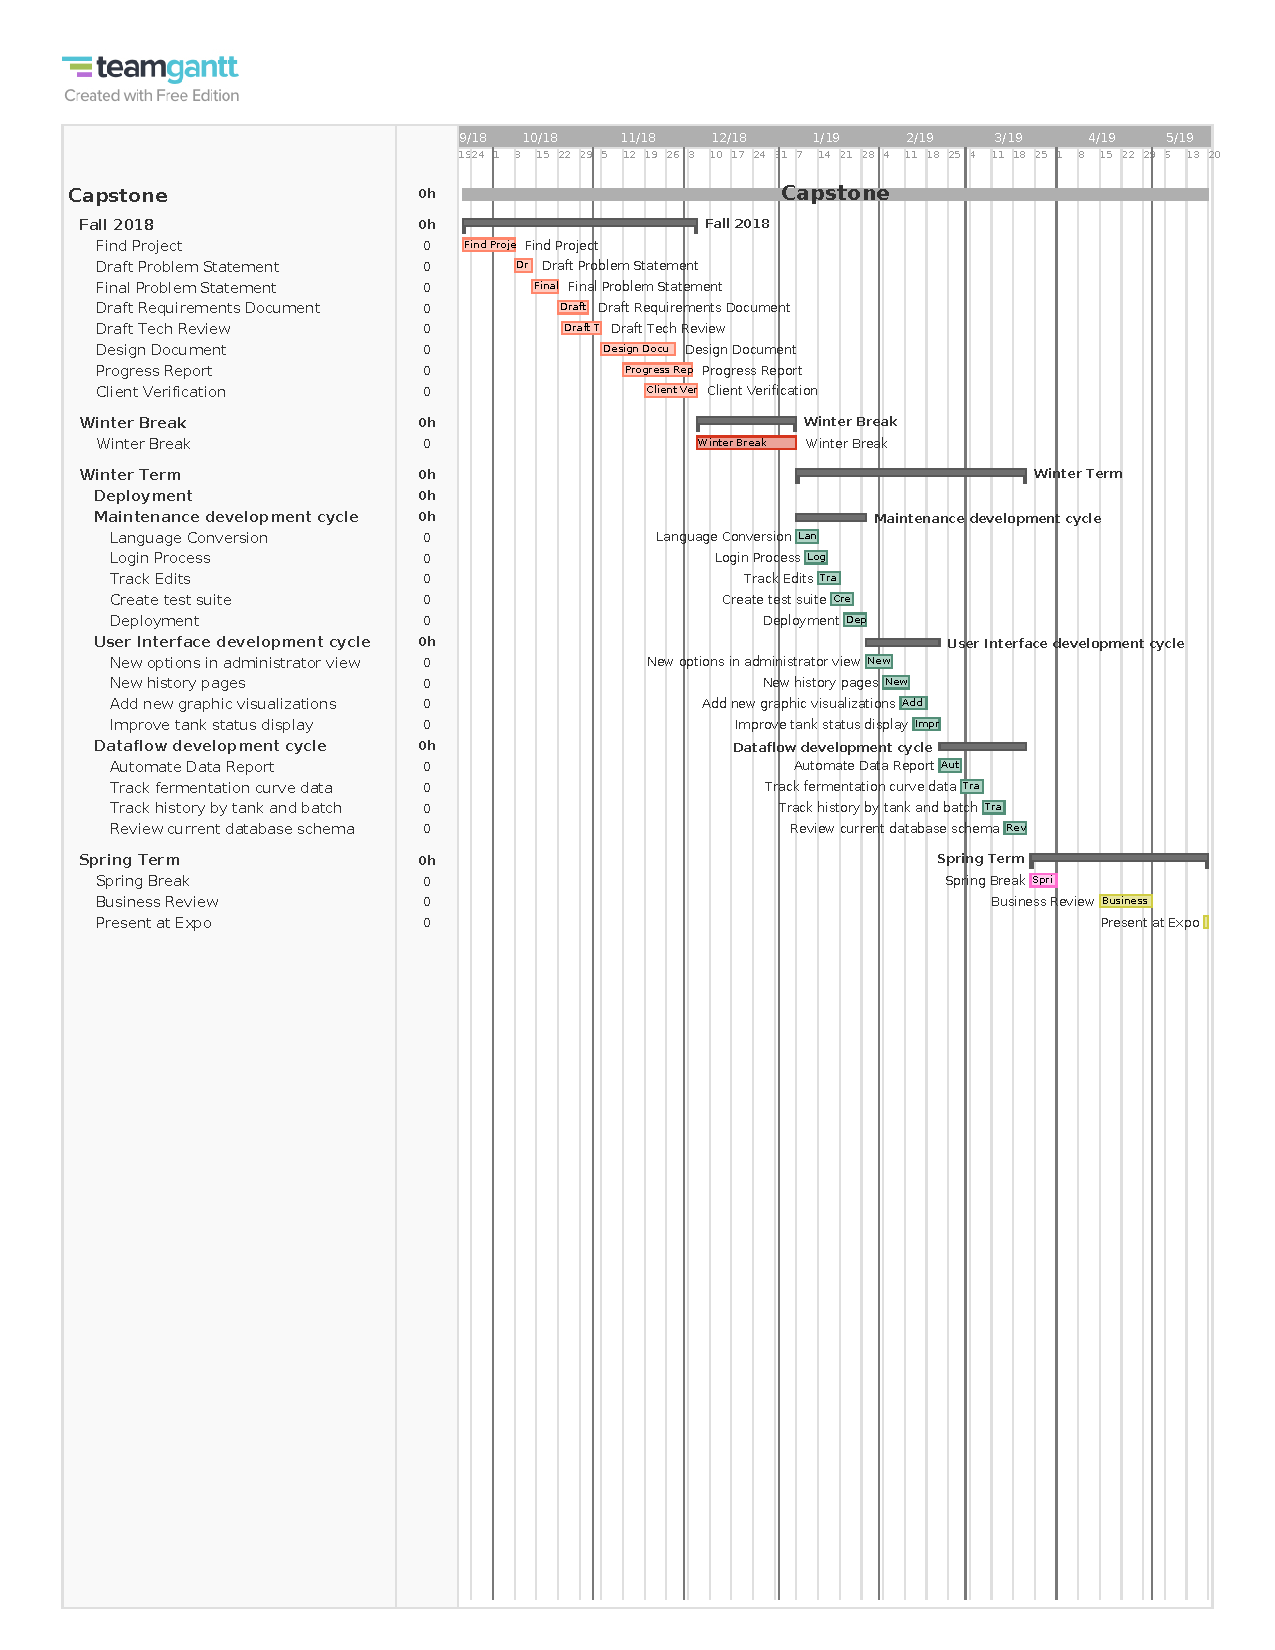
\includepdf[pages=-]{Capstone.pdf}
\end{document}
